\documentclass[titlepage, a4paper]{article}
\usepackage[swedish]{babel}
\usepackage[utf8]{inputenc}
\usepackage{graphicx}
\usepackage{color}
\usepackage{mathtools}
\usepackage{etoolbox}

% Sidformat
\usepackage{a4wide}

% Fixa Appendix-titlar
\usepackage[titletoc,title]{appendix}

% Bättre bildtexter
\usepackage[margin=10pt,font=small,labelfont=bf,labelsep=endash]{caption}

\usepackage{graphicx,epstopdf}
\usepackage{listings}
\epstopdfsetup{suffix=}
\DeclareGraphicsExtensions{.ps}
\DeclareGraphicsRule{.ps}{pdf}{.pdf}{`ps2pdf -dEPSCrop -dNOSAFER #1 \noexpand\OutputFile}

\lstset{literate=%
    {å}{{\r{a}}}1
    {ä}{{\"a}}1
    {ö}{{\"o}}1
    {Å}{{\r{A}}}1
    {Ä}{{\"A}}1
    {Ö}{{\"O}}1
}

%% Headers och Footers
\usepackage{fancyhdr}
\pagestyle{fancy}
\lhead{
\includegraphics[scale=0.2]{LinkUniv_sigill_sv.pdf}}
\rhead{Hannes Snögren \\ Alexander Yngve}
%\rhead{\textit{Laboranter:} \\ Hannes Snögren \\ Alexander Yngve}
\chead{TAOP33}
%\lfoot{TAOP33}
%\cfoot{\thepage}
%\rfoot{}

% Enkelt kommando som låter mig attgöra-markera text
\newcommand{\todo}[1] {\textbf{\textcolor{red}{#1}}}

\pagenumbering{roman}

\begin{document}

{\ }\vspace{45mm}

\begin{center}
    \Huge \textbf{Laborationsrapport}
\end{center}
\begin{center}
    \Large Laboration 3
\end{center}

\vspace{250pt}

\begin{center}
    {\large Laboranter}\\[1.5ex]
    \begin{tabular}{|*{3}{p{40mm}|}}
        \hline
        \textbf{Namn} & \textbf{Personnummer} & \textbf{Epostaddress} \\        \hline
        {Hannes Snögren} & {900708-3976} & {hansn314@student.liu.se} \\\hline
        {Alexander Yngve} & {930320-6651} & {aleyn573@student.liu.se} \\\hline
        \hline
    \end{tabular}
\end{center}
\newpage

\newpage
\section{Inledning}

Vi har blivit tilldelade laborationsuppgift 13 i kursen TAOP33 vid Linköpings universitet. Vi använde programmet VINEOPT av Kaj Holmberg för att lösa problemet.

\section{Uppgift}

Problemet lyder enligt följande.
Ett företag har fyra fabriker som producerar identiska varor. Produktionskostnad och maxproduktion varierar mellan fabrikerna enligt tabell \ref{fabrik-egenskaper}. Företaget har också fem regionala lager med varierande efterfrågan och försäljningspris enligt tabell \ref{lager-egenskaper}.

\begin{table}[h!]
    \centering
    \begin{tabular}{ | l | l | l | l | l | }
        \hline
        {\textbf{Fabrik}} & {$F_{1}$} & {$F_{2}$} & {$F_{3}$} & {$F_{4}$} \\\hline
        {\textbf{Produktionskostnad} (kr/enhet)} & {25} & {27} & {26} & {28} \\\hline
        {\textbf{Maxkapacitet} (enheter)} & {150} & {200} & {175} & {100} \\\hline
    \end{tabular}
    \caption{Fabrikernas egenskaper.} \label{fabrik-egenskaper}
\end{table}

\begin{table}[h!]
    \centering
    \begin{tabular}{ | l | l | l | l | l | l | }
        \hline
        {\textbf{Lager}} & {$L_{1}$} & {$L_{2}$} & {$L_{3}$} & {$L_{4}$} & {$L_{5}$} \\\hline
        {\textbf{Försäljningspris} (kr/enhet)} & {34} & {32} & {31} & {30} & {31} \\\hline
        {\textbf{Efterfrågan} (enheter)} & {80} & {110} & {150} & {100} & {150} \\\hline
    \end{tabular}
    \caption{Regionallagrens egenskaper.} \label{lager-egenskaper}
\end{table}

De tillverkade produkterna skall transporteras från fabrikerna till lagren till en kostnad angiven i tabell \ref{transportkostnader}.

\begin{table}[h!]
    \centering
    \begin{tabular}{ | l | l | l | l | l | l | }
        \hline
        {} & {$L_{1}$} & {$L_{2}$} & {$L_{3}$} & {$L_{4}$} & {$L_{5}$} \\\hline
        {$F_{1}$} & {3} & {1} & {5} & {7} & {7} \\\hline
        {$F_{2}$} & {9} & {7} & {8} & {4} & {5} \\\hline
        {$F_{3}$} & {5} & {4} & {6} & {8} & {6} \\\hline
        {$F_{4}$} & {4} & {5} & {6} & {9} & {7} \\\hline
    \end{tabular}
    \caption{Transportkostnader från fabrik till lager angivet i kr/enhet.} \label{transportkostnader}
\end{table}

Utöver de givna tabellerna finns det 5 givna villkor.

\begin{enumerate}
\item{Mellan fabrik 2 och lager 3 finns ett alternativt transportsätt som bara kostar 3 kr/enhet. Det går dock bara att transportera 25 enheter till denna förmånliga kostnad.} \label{bivillkor1}
\item{Lager 5 måste få hela sin efterfrågan tillgodosedd.} \label{bivillkor2}
\item{Lager 4 måste få minst 80 enheter.} \label{bivillkor3}
\item{Varje fabrik måste tillverka minst 60 enheter.} \label{bivillkor4}
\item{Bolaget tillverkar inte en vara som inte kommer att ge vinst om den inte är nödvändig för att uppfylla övriga krav.} \label{bivillkor5}
\end{enumerate}


\subsection{Deluppgift $a$}

Planera företagets produktion och transport av varor så att största möjliga vinst uppnås.

\subsection{Deluppgift $b$}

Företaget gör en noggrannare analys av kostnadsstrukturen i fabrik 2. Man kommer fram till att de 50 först tillverkade enheterna kostar 28 kr/enhet att tillverka, enhet 51 till 150 kostar 25 kr/enhet att tillverka och enhet 151-200 kostar 28 kr/enhet att tillverka. Hur förändras lösningen? Förändras vinsten?

\subsection{Deluppgift $c$}

En ny transportör erbjuder sig att transportera varor mellan fabrik 3 och lager 3. Vilket pris är det högsta företaget kan tänka sig att betala för att denna transport skall bli lönande för företaget?

\section{Problemuppställning}

Vi identifierar problemet som ett minkostnadsproblem i en tudelad acyklisk riktad graf. Vi identifierar noderna $F_{1}$, $F_{2}$, $F_{3}$ och $F_{4}$ för respektive fabrik och noderna $L_{1}$, $L_{2}$, $L_{3}$, $L_{4}$ och $L_{5}$ för respektive lager.

\begin{figure}[h!]
    \centerline{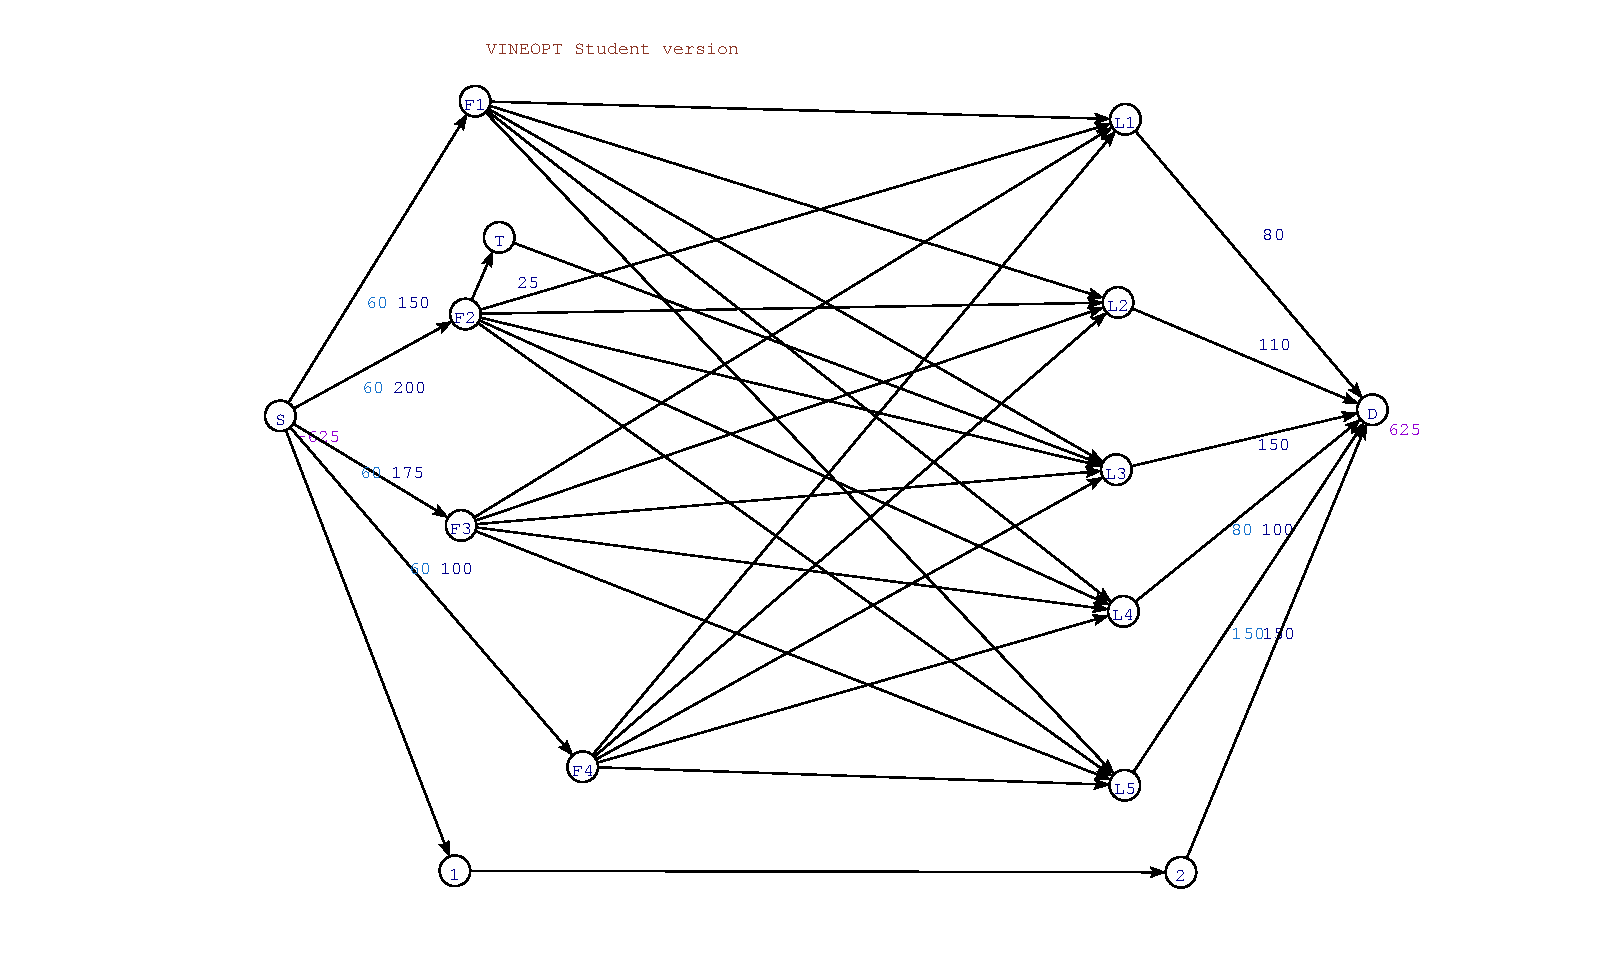
\includegraphics[scale=0.65]{laborationsuppgift_13a_original.ps}}
    \caption{Den identifierade grafen}
\end{figure}

Vi vill att bågkostnaderna i grafen ska innehålla både transportkostnader och kostnad vid försäljning. Vi ställer upp produktionskostnader och försäljningspris som radmatriser respektive kolumnmatriser och upprepar dessa 4 respektive 5 gånger så att vi får $4x5$-matriserna $P$ och $F$. Genom att subtrahera $F$ från $P$ och addera transportkostnadedsmatrisen $T$ från tabell \ref{transportkostnader} får vi så totalkostnadsmatrisen $R$ vars värden vi för in som kostnader på bågarna i grafen.

\begin{displaymath}
P - F + T = R
\end{displaymath}
\begin{displaymath}
\Leftrightarrow
\begin{pmatrix}
     {25} & {25} & {25} & {25} & {25} \\
     {27} & {27} & {27} & {27} & {27} \\
     {26} & {26} & {26} & {26} & {26} \\
     {28} & {28} & {28} & {28} & {28} \\
\end{pmatrix}
-
\begin{pmatrix}
    {34} & {32} & {31} & {30} & {31} \\
    {34} & {32} & {31} & {30} & {31} \\
    {34} & {32} & {31} & {30} & {31} \\
    {34} & {32} & {31} & {30} & {31} \\
\end{pmatrix}
+
\begin{pmatrix}
    {3} & {1} & {5} & {7} & {7} \\
    {9} & {7} & {8} & {4} & {5} \\
    {5} & {4} & {6} & {8} & {6} \\
    {4} & {5} & {6} & {9} & {7} \\
\end{pmatrix}
\end{displaymath}
\begin{displaymath}
=
\begin{pmatrix}
    {-6} & {-6} & {-1} & {2} & {1} \\
    {2} & {2} & {4} & {1} & {1} \\
    {-3} & {-2} & {1} & {4} & {1} \\
    {-2} & {1} & {3} & {7} & {4} \\
\end{pmatrix}
\end{displaymath}

Notera att vi använder kostnad, inte vinst i våra beräkningar vilket leder till att vinst representeras av ett negativt nummer. Alltså är de varor som transporteras via bågar med positiv kostnad i kostnadsmatrisen $R$ förlustaffärer.

Startnoden $S$ har en kapacitet som motsvarar summan av fabrikernas maxkapaciteter. Eftersom summan av fabrikrenas maxkapaciteter är större än summan av lagrens efterfrågan, fungerar endast nätet om slutnoden $D$ har en efterfrågan lika stor som kapaciteten i $S$.

Vi sätter de övre begränsningarna på bågarna från $S$ till $F_{n}$ till fabrikernas maxkapacitet och de undre till 60 enheter enligt villkor \ref{bivillkor4}. Vi sätter motsvarande begränsningar för lagren mellan $L_{n}$ och $D$.

Noderna $1$ och $2$ finns endast för estetiska skäl och bågarna däremellan har en kostnad på 0 kr. Det innebär att förutom det flöde som krävs för att uppfylla övriga villkor, kommer endast lönsamt flöde gå genom resten av grafen i enlighet med villkor \ref{bivillkor5}.

Noden $T$ är ett substitut för en parallell båge och är det alternativa, billigare transportsättet mellan $F_{2}$ och $L_{3}$ givet i villkor \ref{bivillkor1}. Vi får kostnaden för den genom att beräkna $p_{2}-f_{3}+3$.

\section{Lösning deluppgift $a$}

För att ta reda på största möjliga vinst för företaget, löser vi den graf vi ritat upp. Lösningen illustreras i figur \ref{uppgifta-losning}. Svaret blir att största möjliga vinst är 715 kr med ettflöde enligt tabell \ref{uppgifta-flode}.

\begin{figure}[h!]
\centerline{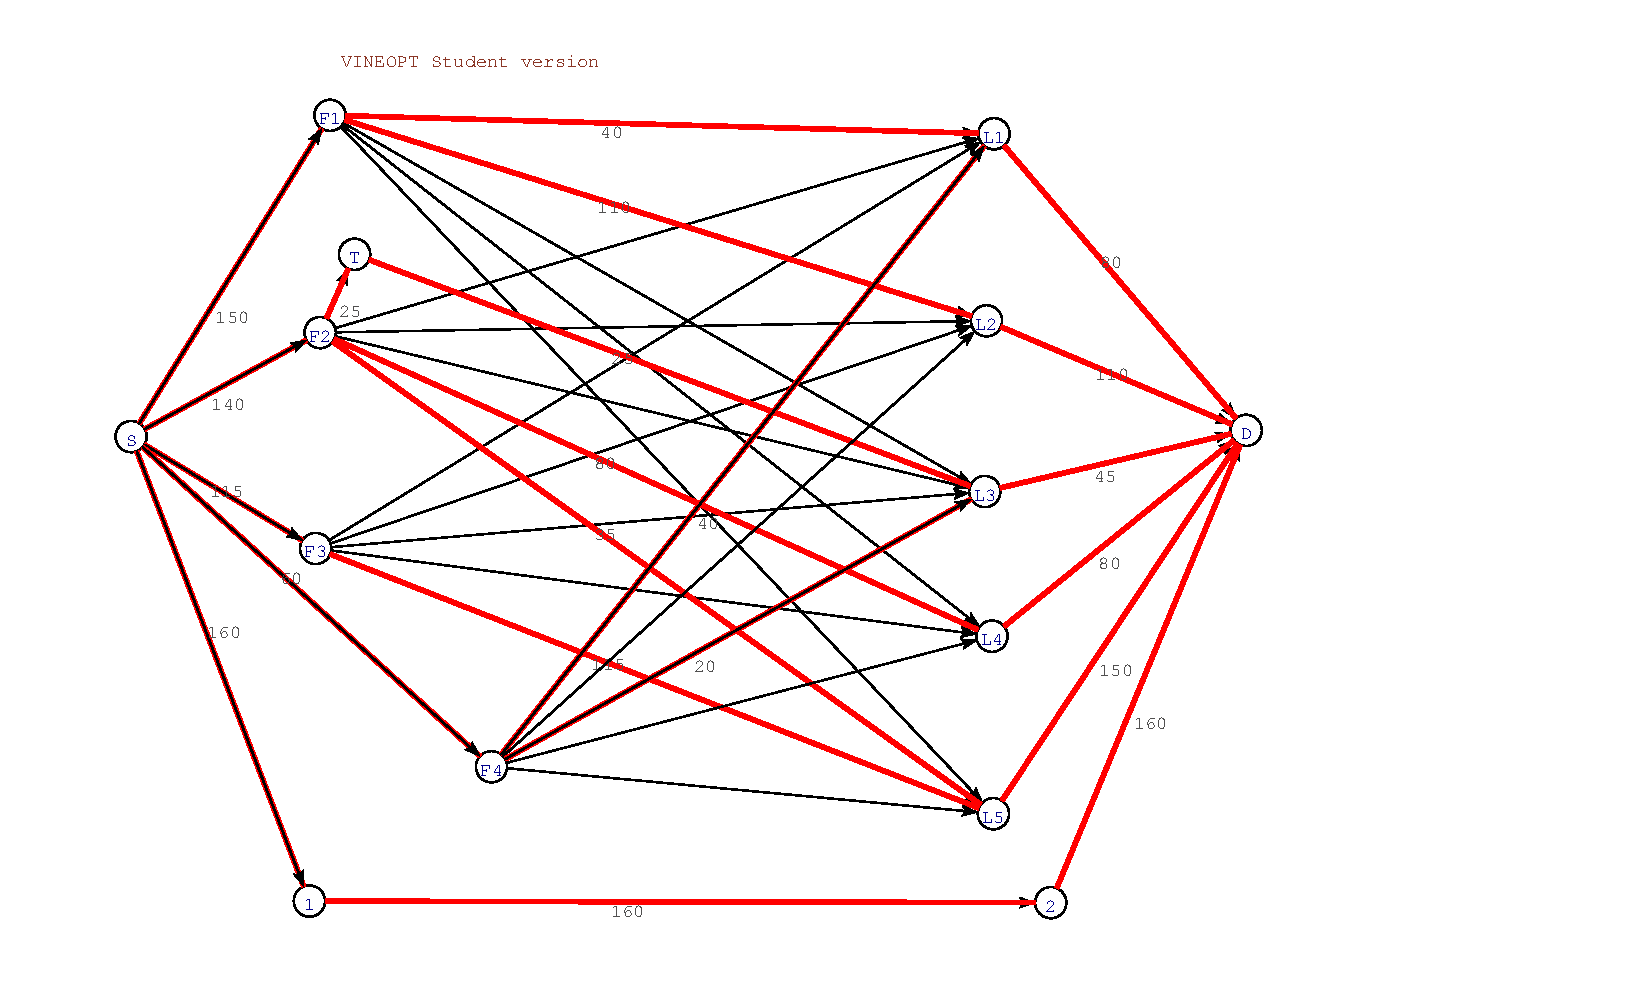
\includegraphics[scale=0.65]{laborationsuppgift_13a_solved.ps}}
\caption{Lösning deluppgift $a$} \label{uppgifta-losning}
\end{figure}

\begin{table}[h!]
    \centering
    \begin{tabular}{ | l | l | l | l | l | l | }
        \hline
        {} & {$L_{1}$} & {$L_{2}$} & {$L_{3}$} & {$L_{4}$} & {$L_{5}$} \\\hline
        {$F_{1}$} & {20} & {110} & {20} & {} & {} \\\hline
        {$F_{2}$} & {} & {} & {25} & {80} & {16} \\\hline
        {$F_{3}$} & {} & {} & {} & {} & {134} \\\hline
        {$F_{4}$} & {60} & {} & {} & {} & {} \\\hline
    \end{tabular}
    \caption{Transportkostnader från fabrik till lager angivet i kr/enhet.} \label{uppgifta-flode}
\end{table}

\newpage

\section{Lösning deluppgift $b$}

För att lösa uppgiften måste vi modifiera grafen. Vi lägger till noderna $F_{2a}$, $F_{2b}$ och $F_{2c}$ mellan $S$ och $F_{2}$. Vi ger bågarna mellan de nya noderna och $F_{2}$ kostnader och gränser för maximalt och minimalt flöde enligt tabell \ref{uppgiftb-bagar} för att uppfylla de nya villkoren.

\begin{table}[h!]
    \centering
    \begin{tabular}{ | l | l | l | l | }
        \hline
        {\textbf{Startnod}} & {\textbf{Kostnad}} & {\textbf{Maxflöde}} & {\textbf{Minflöde}} \\\hline
        {$F_{2a}$} & {1} & {50} & {50} \\\hline
        {$F_{2b}$} & {-2} & {100} & {10} \\\hline
        {$F_{2c}$} & {1} & {$\infty$} & {0} \\\hline
    \end{tabular}
    \caption{Värden för nya bågar med $F_{2}$ som slutnod.} \label{uppgiftb-bagar}
\end{table}

\begin{figure}[h!]
\centerline{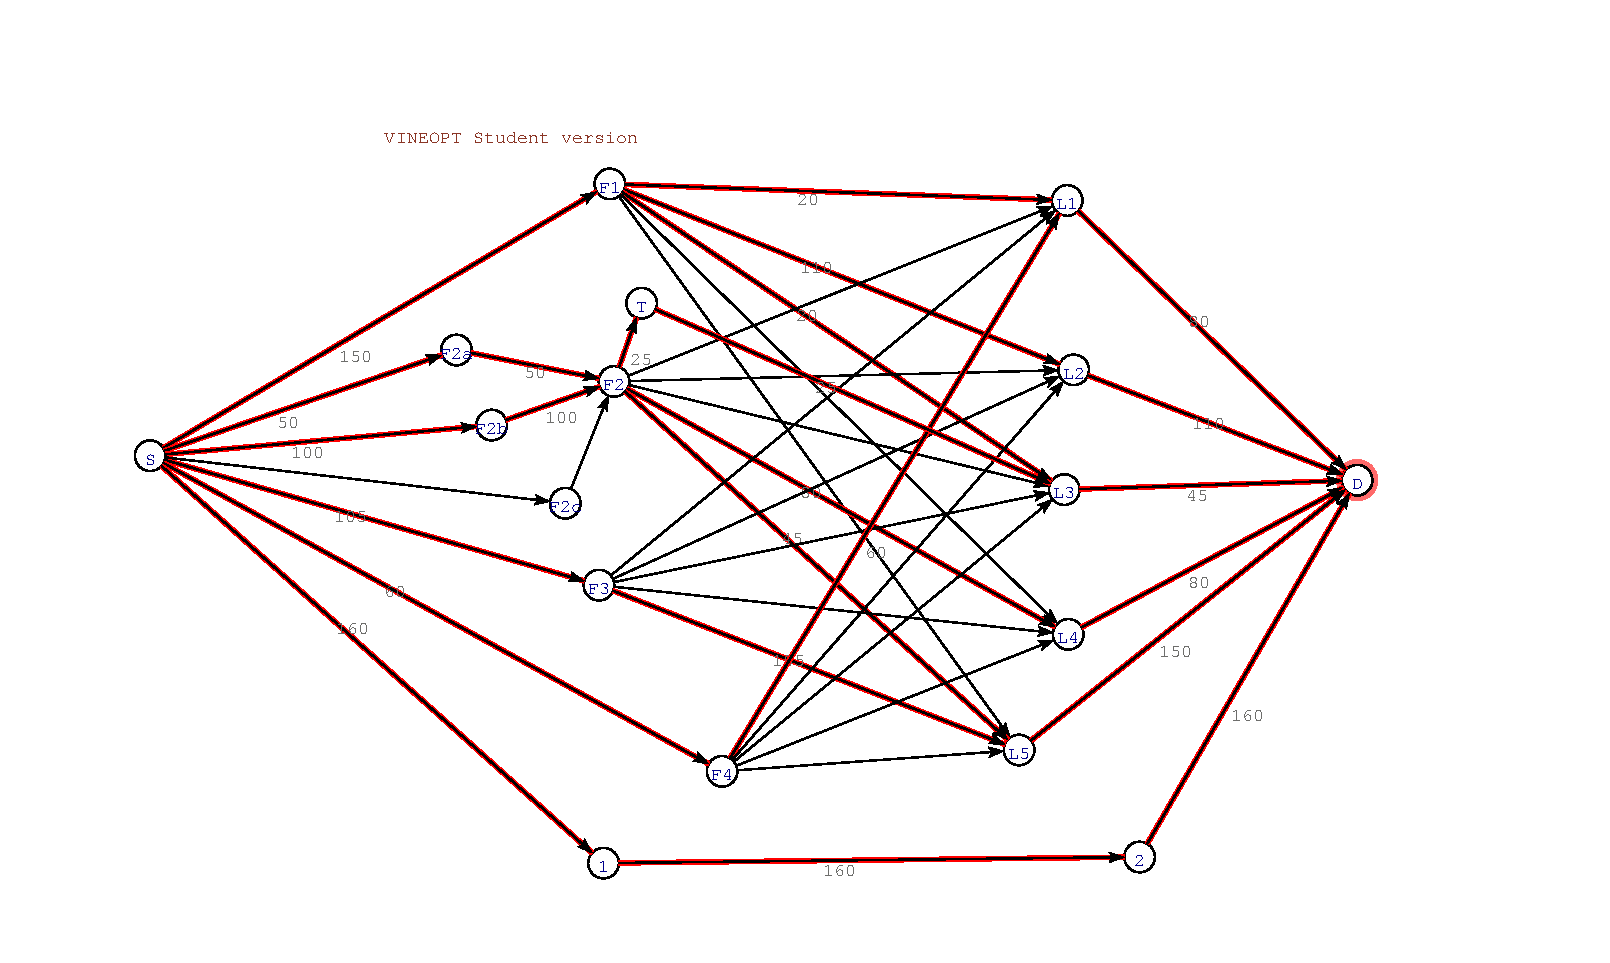
\includegraphics[scale=0.65]{laborationsuppgift_13b_solved.ps}}
\caption{Lösning deluppgift $b$} \label{uppgiftb-graf}
\end{figure}

Vi löser sedan grafen och får ett resultat enligt figur \ref{uppgiftb-graf}. Lösningen ger en vinst på 865 kr med ett flöde enligt tabell \ref{uppgiftb-flode}.

\begin{table}[h!]
    \centering
    \begin{tabular}{ | l | l | l | l | l | l | }
        \hline
        {} & {$L_{1}$} & {$L_{2}$} & {$L_{3}$} & {$L_{4}$} & {$L_{5}$} \\\hline
        {$F_{1}$} & {20} & {110} & {20} & {} & {} \\\hline
        {$F_{2}$} & {} & {} & {25} & {80} & {45} \\\hline
        {$F_{3}$} & {} & {} & {} & {} & {105} \\\hline
        {$F_{4}$} & {60} & {} & {} & {} & {} \\\hline
    \end{tabular}
    \caption{Transportkostnader från fabrik till lager angivet i kr/enhet.} \label{uppgiftb-flode}
\end{table}

\section{Lösning deluppgift $c$}

Genom att studera matrisen $R$ ser vi att kostnaden är $1$ kr/enhet för att producera, transportera och sälja en vara från $F_{3}$ till $L_{3}$. För att det ska vara lönsamt måste kostnaden vara $<0$ kr och alltså måste vi begära ett pris $<5$ kr/enhet.

\newpage
\begin{appendices}
{\ }\vspace{1mm}
\section{MATLAB-script för lösning av kostnadsmatriser}
\lstinputlisting{kostnad.m}
\end{appendices}

\end{document}
